\begin{enumerate}
\item In \figref{fig:Fig_1}, two concentric circles with centre $O$, have radii $21 cm$ and $42 cm$. If $\angle AOB = 60\degree$, find the area of the shaded region.
\begin{figure}[H]
    \centering
    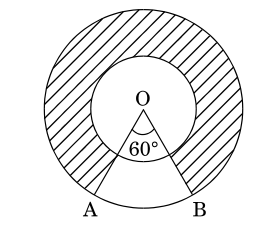
\includegraphics[width=\columnwidth]{figs/geo.png}
    \caption{Circle $AOB$ }
    \label{fig:Fig_1}
\end{figure}

\item A moving boat is observed from the top of a $150m$ high cliff moving away from the cliff. The angle of depression of the boat changes from $60\degree$ to $45\degree$ in $2$ minutes. Find the speed of the boat in m/min.

\item There are two poles, one each on either bank of a river just opposite to each other. One pole is $60m$ high. From the top of this pole, the angle of depression of the top and foot of the other pole are $30\degree$ and $60\degree$respectively. Find the width of the river and height of the other pole.

\item A cone of height $24 cm$ and radius of base $6 cm$ is made up of modelling clay. A child reshapes it in the form of a sphere. Find the radius of the sphere and hence find the surface area of this sphere.

\item A farmer connects a pipe of internal diameter $20 cm$ from a canal into a cylindrical tank in his field which is $10 m$ in diameter and $2 m$ deep. If water flows through the pipe at the rate of $3 km/hr$, in how much time will the tank be filled ?

\item Find the dimensions of a rectangular park whose perimeter is $60 m$ and area $200 m^2$.

\item A container opened at the top and made up of a metal sheet, is in the form of a frustum of a cone of height $16$ cm with radii of its lower and upper ends as $8$ cm and $20$ cm respectively. Find the cost of milk which can completely fill the container, at the rate of \rupee $50$ per litre. Also find the cost of metal sheet used to make the container, if it costs \rupee$ 10$ per $100 cm^2$. Take$\brak{\pi = 3.14}$

\item Two poles of equal heights are standing opposite to each other on either side of the road which is $80 m$ wide. From a point $P$ between them on the road, the angle of elevation of the top of a pole is $60\degree$ and the angle of depression from the top of the other pole of point $P$ is $30\degree$. Find the heights of the poles and the distance of the point $P$ from the poles.

\item Amit, standing on a horizontal plane, finds a bird flying at a distance of $200 m$ from him at an elevation of $30\degree$. Deepak standing on the roof of a $50 m$ high building, finds the angle of elevation of the same bird to be $45\degree$. Amit and Deepak are on opposite sides of the bird. Find the distance of the bird from Deepak.

\item From a point $P$ on the ground, the angle of elevation of the top of a tower is $30\degree$ and that of the top of the flag-staff fixed on the top of the tower is $\sqrt{5}$. If the length of the flag-staff is $5 m$, find the height of the tower. (Use $\sqrt{3}= 1.732$).


\item A solid iron pole consists of a cylinder of height $220 cm$ and base diameter $24 cm$, which is surmounted by another cylinder of height $60 cm$ and radius $8 cm$. Find the mass of the pole, given that $1 cm^3$ of iron has approximately $8 gm$ mass. (use $ \pi =3.14$)

\item A solid is in the form of a cylinder with hemispherical ends. The total
height of the solid is $20 cm$ and the diameter of the cylinder is $7 cm$. Find the total volume of the solid. (use $\pi = \frac{22}{7}$). 

\item Two spheres of same metal weigh $1 kg $and $7 kg$. The radius of the smaller sphere is $3 cm$. The two spheres are melted to form a single big sphere. Find the diameter of the new sphere.

\item A right cylindrical container of radius $6 cm$ and height $15 cm$ is full of ice-cream, which has to be distributed to $10$ children in equal cones having hemispherical shape on the top. If the height of the conical portion is four times its base radius, find the radius of the ice-cream cone.

\item In a triangle, if square of one side is equal to the sum of the squares of the other two sides, then prove that the angle opposite the first side is a right angle.

\item Prove that the ratio of the areas of two similar triangles is equal to the ratio of the squares on their corresponding sides.

\item If a line is drawn parallel to one side of a triangle to intersect the  other two sides in distinct points, then prove that the other two sides are divided in the same ratio.



\item In  \figref{fig:Figh_4}, a square $OABC$ is inscribed in a quadrant $OPBQ$. If $OA = 15 cm$, find the area of the shaded region. (Use $\pi = 3.14$)
\begin{figure}[H]
    \centering
    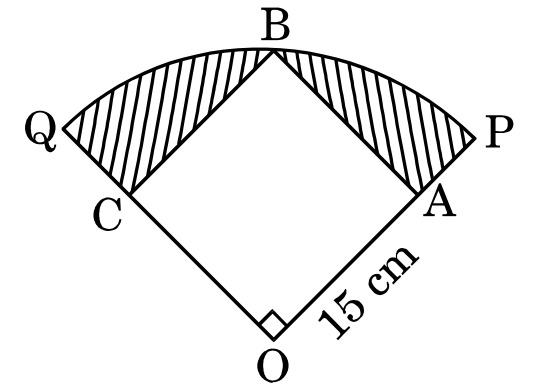
\includegraphics[width=\columnwidth]{figs/img4.jpg}
    \caption{Square $OABC$}
    \label{fig:Figh_4}
\end{figure}

\item In  \figref{fig:Figh_5}, $ABCD$ is a square with side $2\sqrt{2}cm$ and inscribed in a circle. Find the area of the shaded region. (Use $\pi = 3.14$).
\begin{figure}[H]
    \centering
    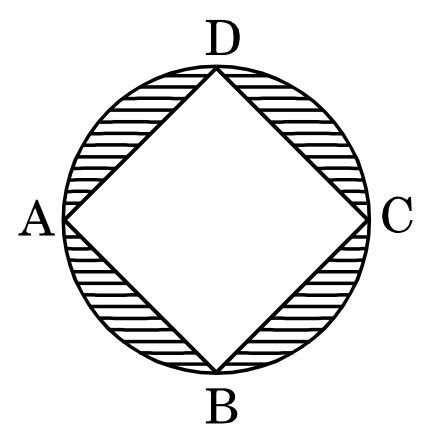
\includegraphics[width=\columnwidth]{figs/img5.jpg}
    \caption{Square $ABCD$ }
    \label{fig:Figh_5}
\end{figure}

\item The shadow of a tower standing on a level ground is found to be $40 m$ longer when the Sun's altitude is $30\degree$ than when it was $60\degree$. Find the height of the tower. $(Given \sqrt{3} = 1.732)$

\item Prove that in a right triangle, the square of the hypotenuse is equal to the sum of the squares of the other two sides.

\item Prove that opposite sides of a quadrilateral circumscribing a circle subtend supplementary angles at the centre of the circle.

\item A pole has to be erected at a point on the boundary of a circular park of diameter $13 m$ in such a way that the difference of its distances from two
diametrically opposite fixed gates $A$ and $B$ on the boundary is $7 m$. Is it possible to do so ? If yes, at what distances from the two gates should the pole be erected ?

\item Water in a canal, $6 m$ wide and $1.5 m$ deep, is flowing with a speed of $10 km/h $. How much area will it irrigate in $30$ minutes if $8 cm$ of standing water is needed?

\item A car has two wipers which do not overlap. Each wiper has a blade of length $21 cm$ sweeping through an angle $120\degree$. Find the total area cleaned at each sweep of the blades. $(Take  \pi=\frac{22}{7})$

\item In \figref{fig:Fig-3}, a decorative block is shown which is made of two solids, a cube and a hemisphere. The base of the block is a cube with edge $6 cm $ and the hemisphere fixed on the top has a diameter of $4.2 cm $. Find
 \begin{enumerate}
 \item  the total surface area of the block.
 \item the volume of the block formed.(Take  $\pi=\frac{22}{7}$)
 \end{enumerate}
\begin{figure}[H]
    \centering
    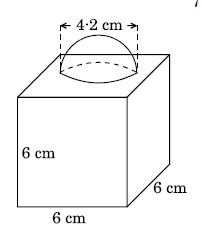
\includegraphics[width=\columnwidth]{figs/image.png}
    \caption{CUBE AND HEMISPHERE}
    \label{fig:Fig-3}
\end{figure}

\item A bucket open at the top is in the form of a frustum of a cone with a capacity of $12308.8 cm^3 $. The radii of the top and bottom circular ends are $20 cm $ and $12 cm $ respectively. Find the height of the bucket and the area of metal sheet used in making the bucket.$(Use \pi=3.17)$


\item In \figref{fig:figppr-2}, three sectors of a circle of radius $7cm$, making angles of $60\degree$,
$80\degree$ and $40\degree$ at the centre are shaded. Find the the area of the shaded region.
\begin{figure}[H]
    \centering
    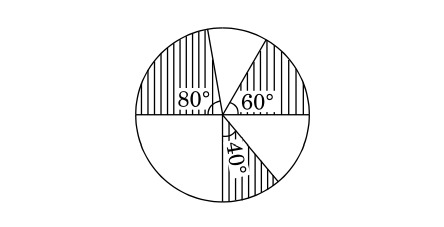
\includegraphics[width=\columnwidth]{figs/Figure_2.png}
    \caption{Circle}
    \label{fig:figppr-2}
\end{figure}

\item A juice seller was serving his customers using glasses as shown in \figref{fig:Figpppr-3} . The inner diameter of the cylindrical glass was $5 cm$ but bottom of the glass had a hemispherical raised portion which reduced the capacity of the glass. If the height of a glass was $10 cm$, find the apparent and actual capacity of the glass. (Use $\pi = 3.14$ )
\begin{figure}[H]
    \centering
    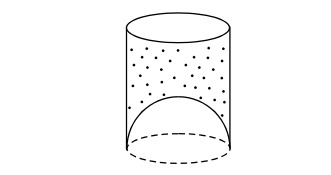
\includegraphics[width=\columnwidth]{figs/Figure_3.png}
    \caption{Hemisphere}
    
    \label{fig:Figpppr-3}
\end{figure}

\item A girl empties a cylindrical bucket full of sand, of base radius $18 cm$ and height $32 cm$ on the floor to form a conical heap of sand. If the height of this conical heap is $24 cm$, then find its slant height correct to one place of decimal.

\item An open metallic bucket is in the shape of a frustum of a cone. If the diameters of the two circular ends of the bucket are $45 cm$ and $25 cm$ and the vertical height of the bucket is $24 cm$, find the area of the metallic sheet used to make the bucket. Also find the volume of the water it can 
hold. (Use $\pi =\frac{22}{7}$)




\end{enumerate}
